%!TEX root = batch-course.tex
%-------------------------------------------------
\section{General multivariate review}
%-------------------------------------------------

\begin{frame}\frametitle{Justification for latent variable methods}

\begin{enumerate}
	\item	High dimensionality in data we collect, e.g. NIR spectra
			\begin{center}
				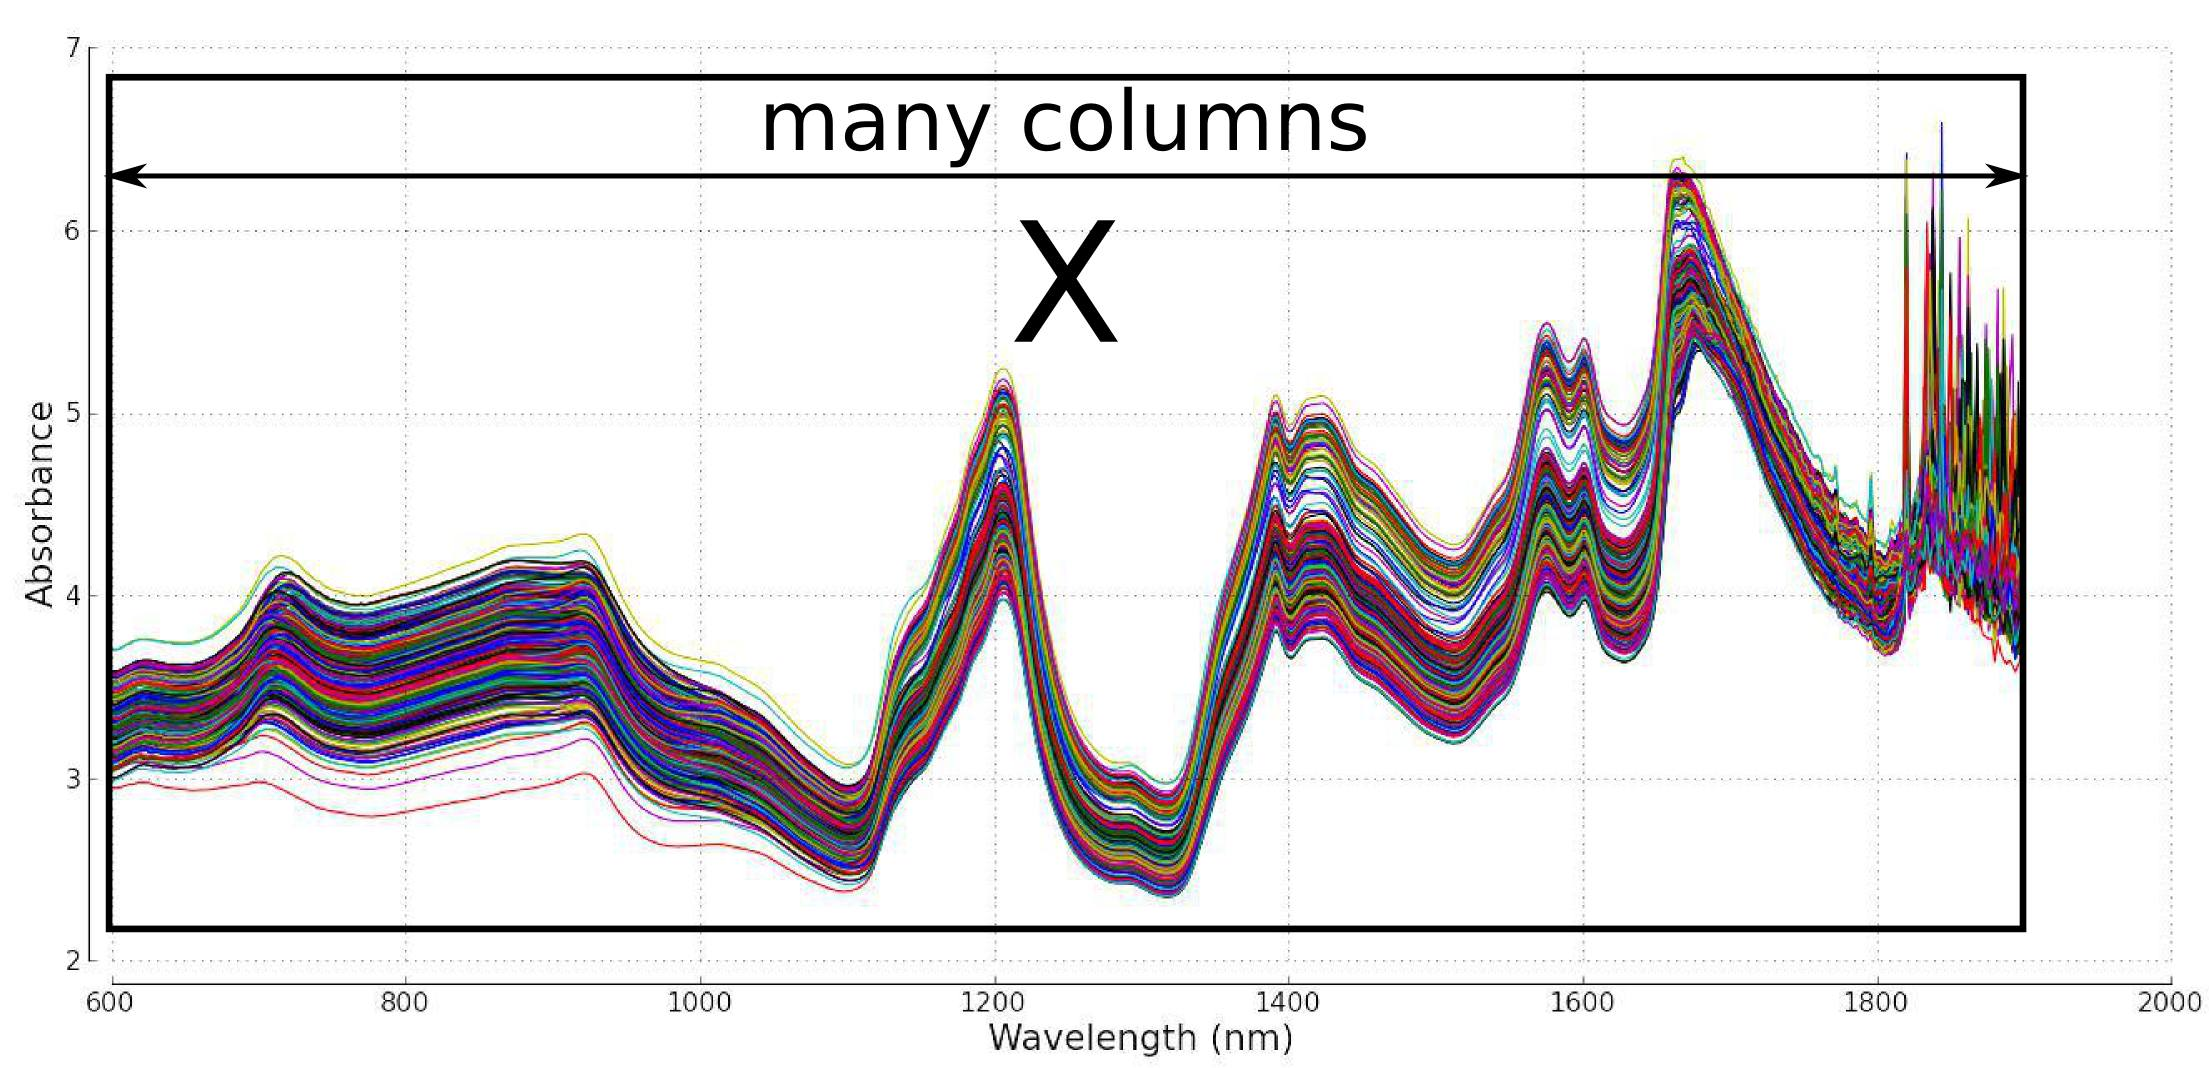
\includegraphics[width=6cm]{images/high-dimensionality-data.jpg}
			\end{center}
			
			
	\item	High correlation between the variables (duplicate info)
			\vspace{6pt}
			\begin{columns}
				\column{.30\textwidth}
				\begin{center}
					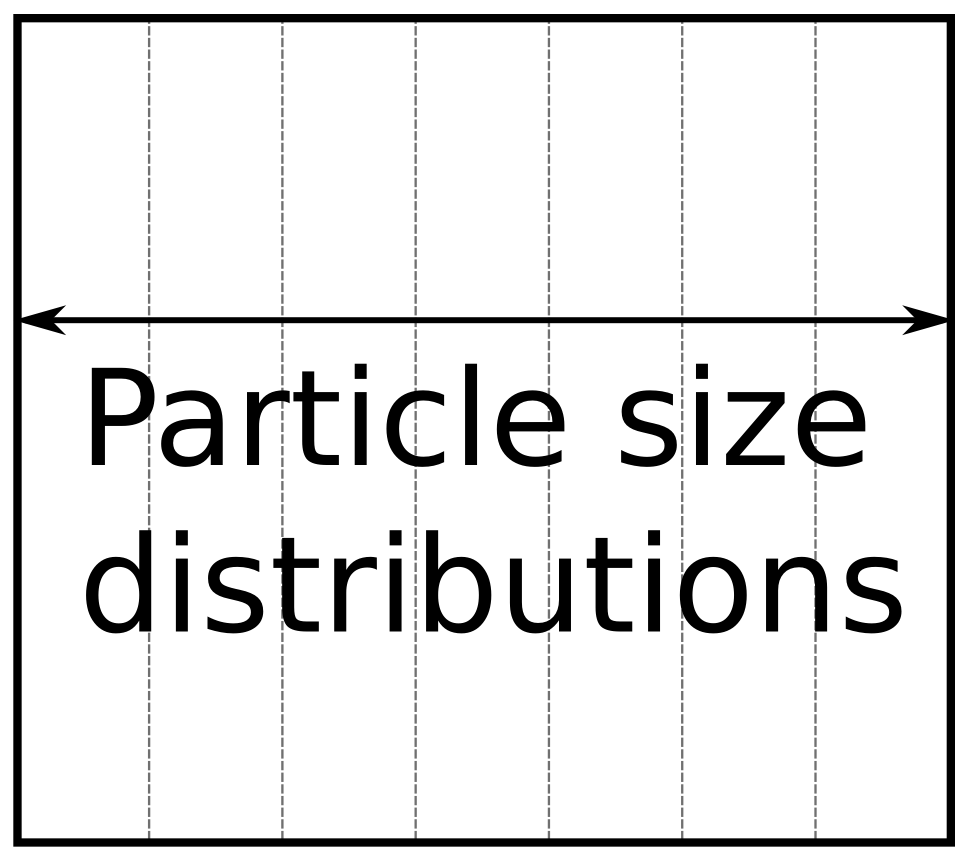
\includegraphics[width=3cm]{images/high-correlation-between-variables.png}
				\end{center}
				
				\column{.7\textwidth}
				Not a bad thing, but ordinary least squares cannot handle high correlations
				\begin{itemize}
					\item	we resort to variable selection					
					\item	we risk omitting important variables
					\item	using all data: get stronger signal from many noisy variables
				\end{itemize}
				
			\end{columns}
			
\end{enumerate}
\end{frame}

\begin{frame}\frametitle{Justification for latent variable methods}

\begin{enumerate}
	\setcounter{enumi}{2}
	\item	Missing data
	
			\begin{center}
				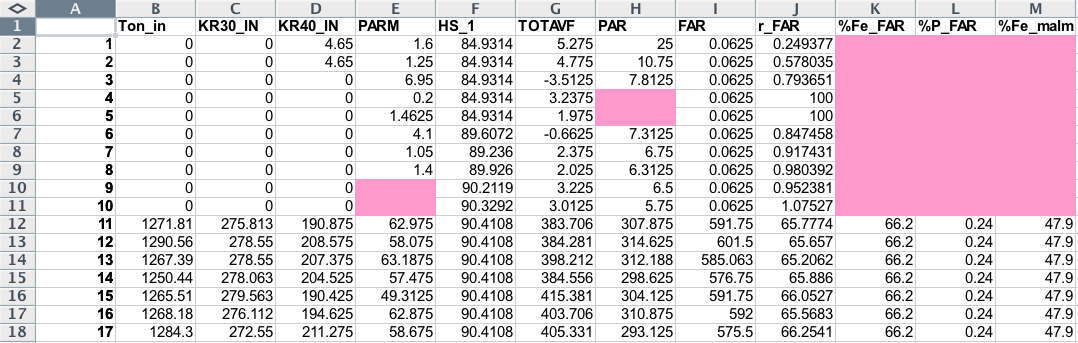
\includegraphics[width=6cm]{images/missing-data.png}
			\end{center}
			
			Batch data sets: usually not an issue for complete, historical batches			
			
	
	\item	Large number of samples
	
			\begin{itemize}
				\item	modern computer hardware
				
				\item	smart algorithms (build models from smaller data groups)
			\end{itemize} 
\end{enumerate}
\end{frame}

\begin{frame}\frametitle{Quick review of multivariate concepts: PCA}

	\begin{block}{Mathematical objective}
		PCA: find me the best summary of my data, \( \mathbf{X} \), with the fewest number of summary variables, called scores, \( \mathbf{T} \).
	\end{block}
	
	\vspace{18pt}

	\begin{center}
		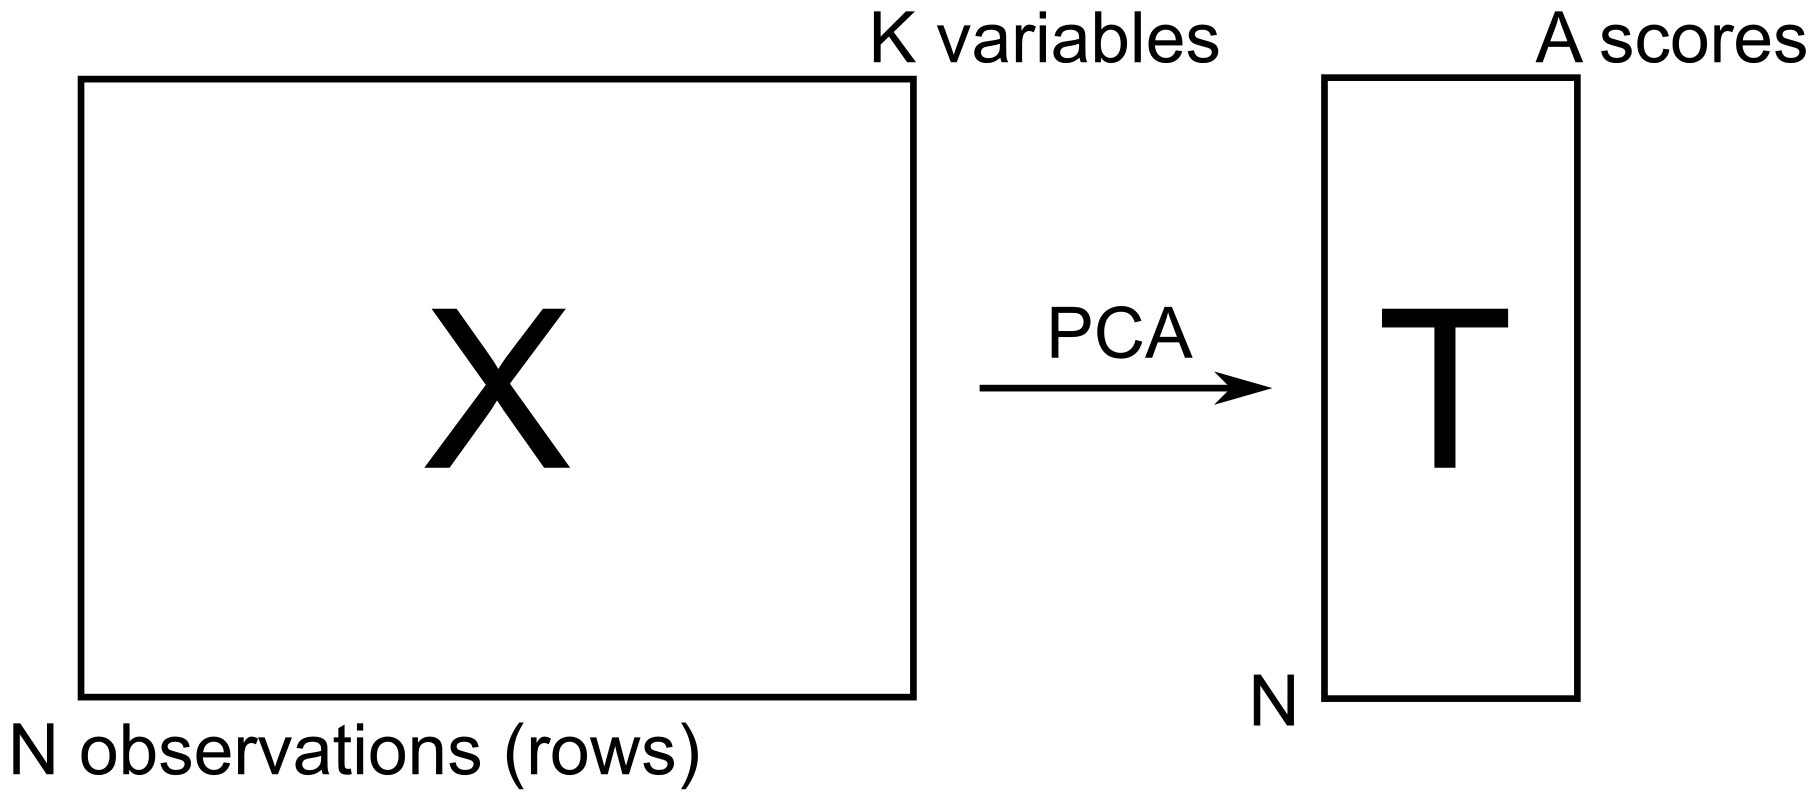
\includegraphics[width=8cm]{images/reduce-data-X-to-scores-T.png}
	\end{center}
	
\end{frame}

\begin{frame}\frametitle{What does PCA do?}

	It finds directions that best explain the data.  Also called
	
	\begin{itemize}
		\item  	``directions of greatest variance''
		\item	``loadings and scores''
		\item	``components''
		\item	``latent variables'' (LVs)
	\end{itemize}

	\begin{center}
		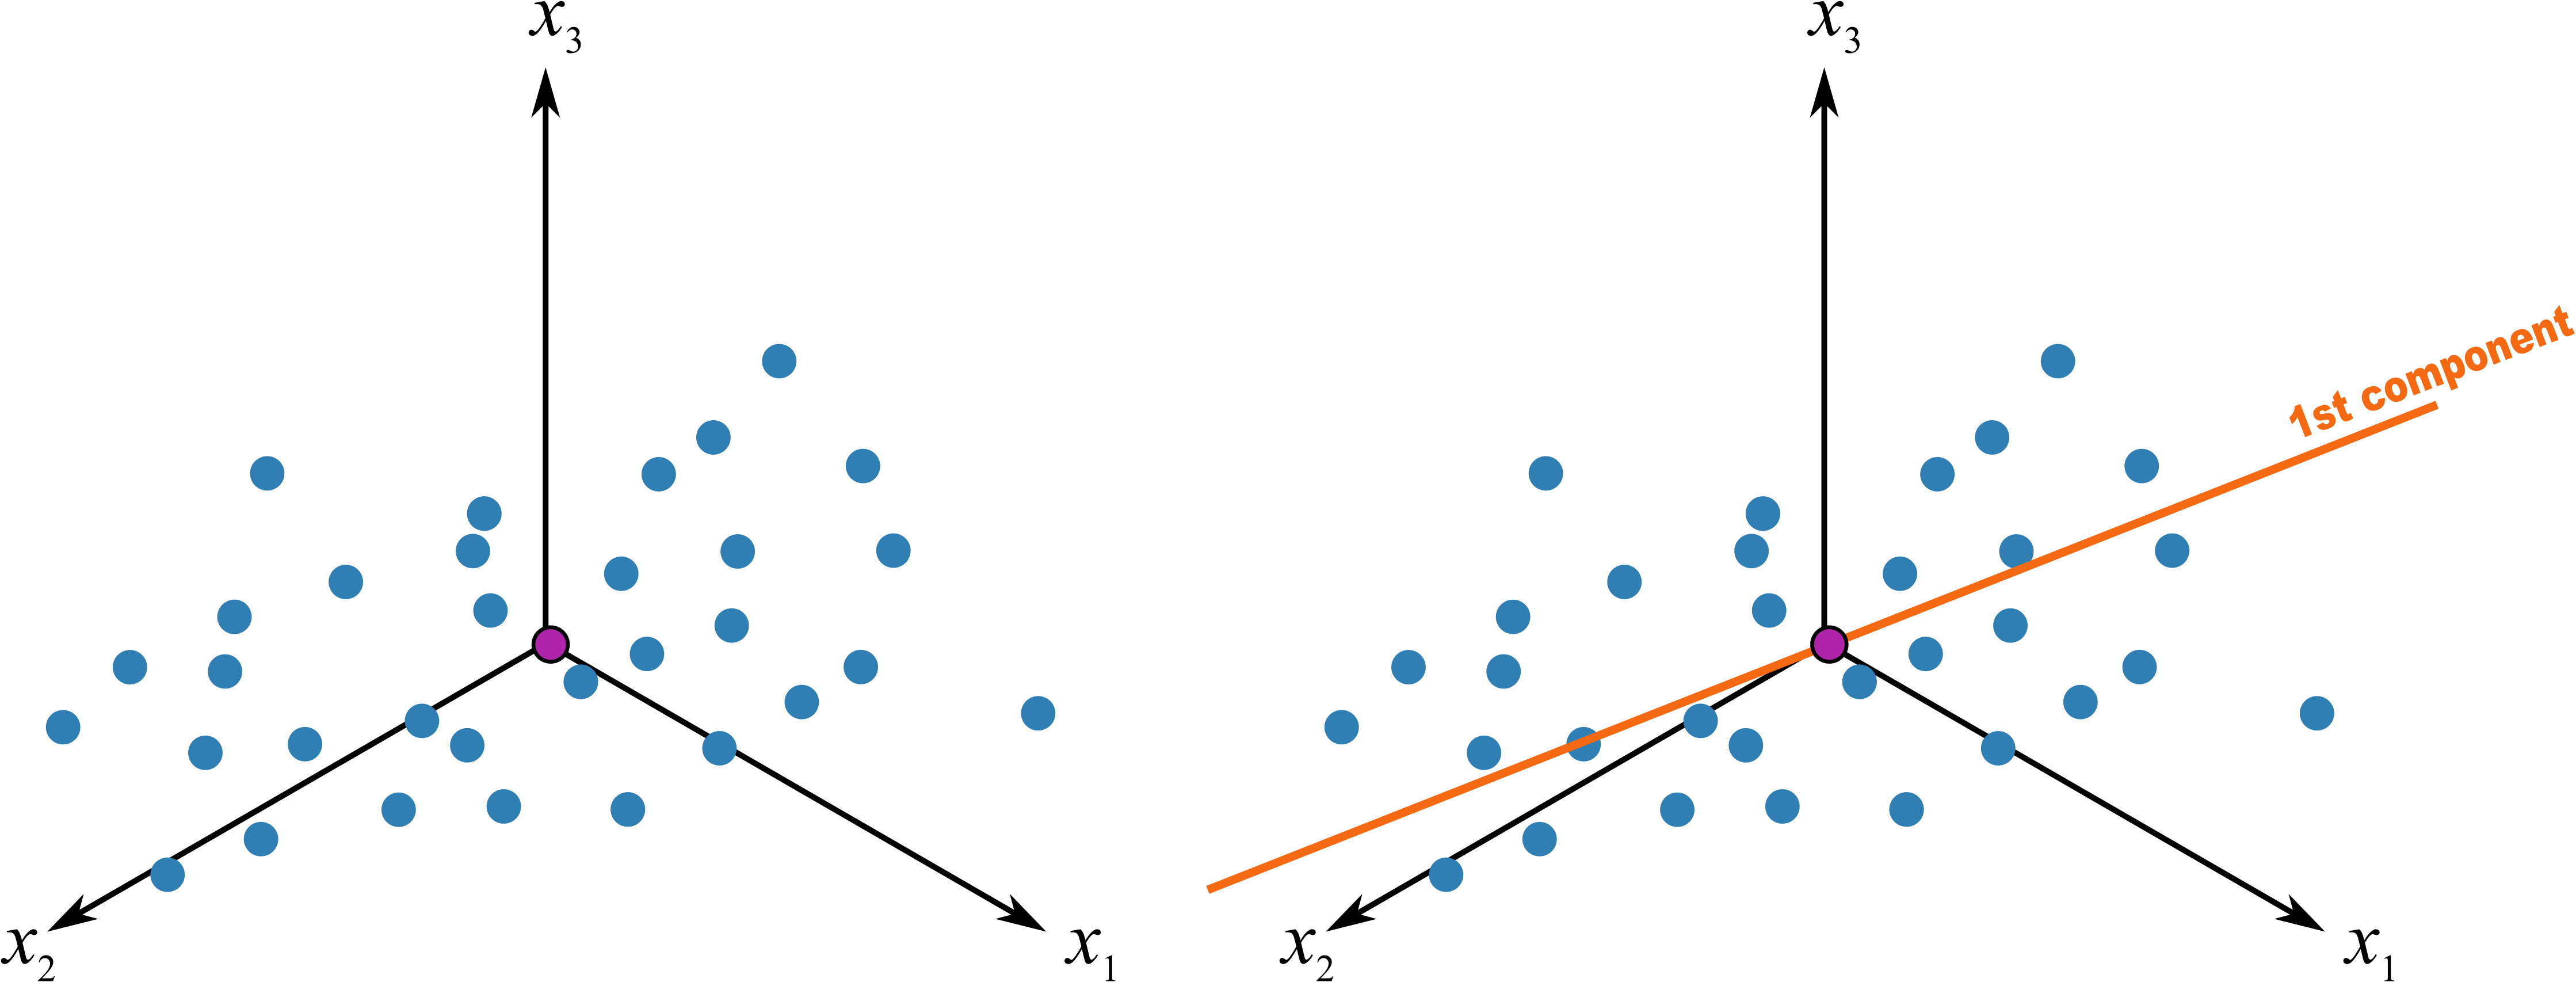
\includegraphics[width=\textwidth]{images/geometric-PCA-3-and-4-centered-with-first-component.png}
		% images/geometric-interpretation-of-PCA.svg
	\end{center}
	
	PCA finds the LVs so that LV1 explains more than LV2, which explains more than LV3, \emph{etc}.
\end{frame}

\begin{frame}\frametitle{What is a latent variable?}

	\textbf{\emph{Example}}: your health
	
	\begin{itemize}
		\item	There isn't a single measurement of ``health''.  It's an abstract concept: 
		
				\begin{itemize}
					\item	blood pressure, cholesterol, blood sugar, temperature, heart rate \emph{etc}
				\end{itemize}				
				
		\item	combine these values in some way (by a trained professional) to come up with some level of ``health''
	\end{itemize}
	
	\pause
	
	{\color{myGreen}{We can do this with any system!}}
\end{frame}

\begin{frame}\frametitle{What is a latent variable?}

	\textbf{\emph{Example}}: room temperature measured at 4 points
	
	\begin{center}
		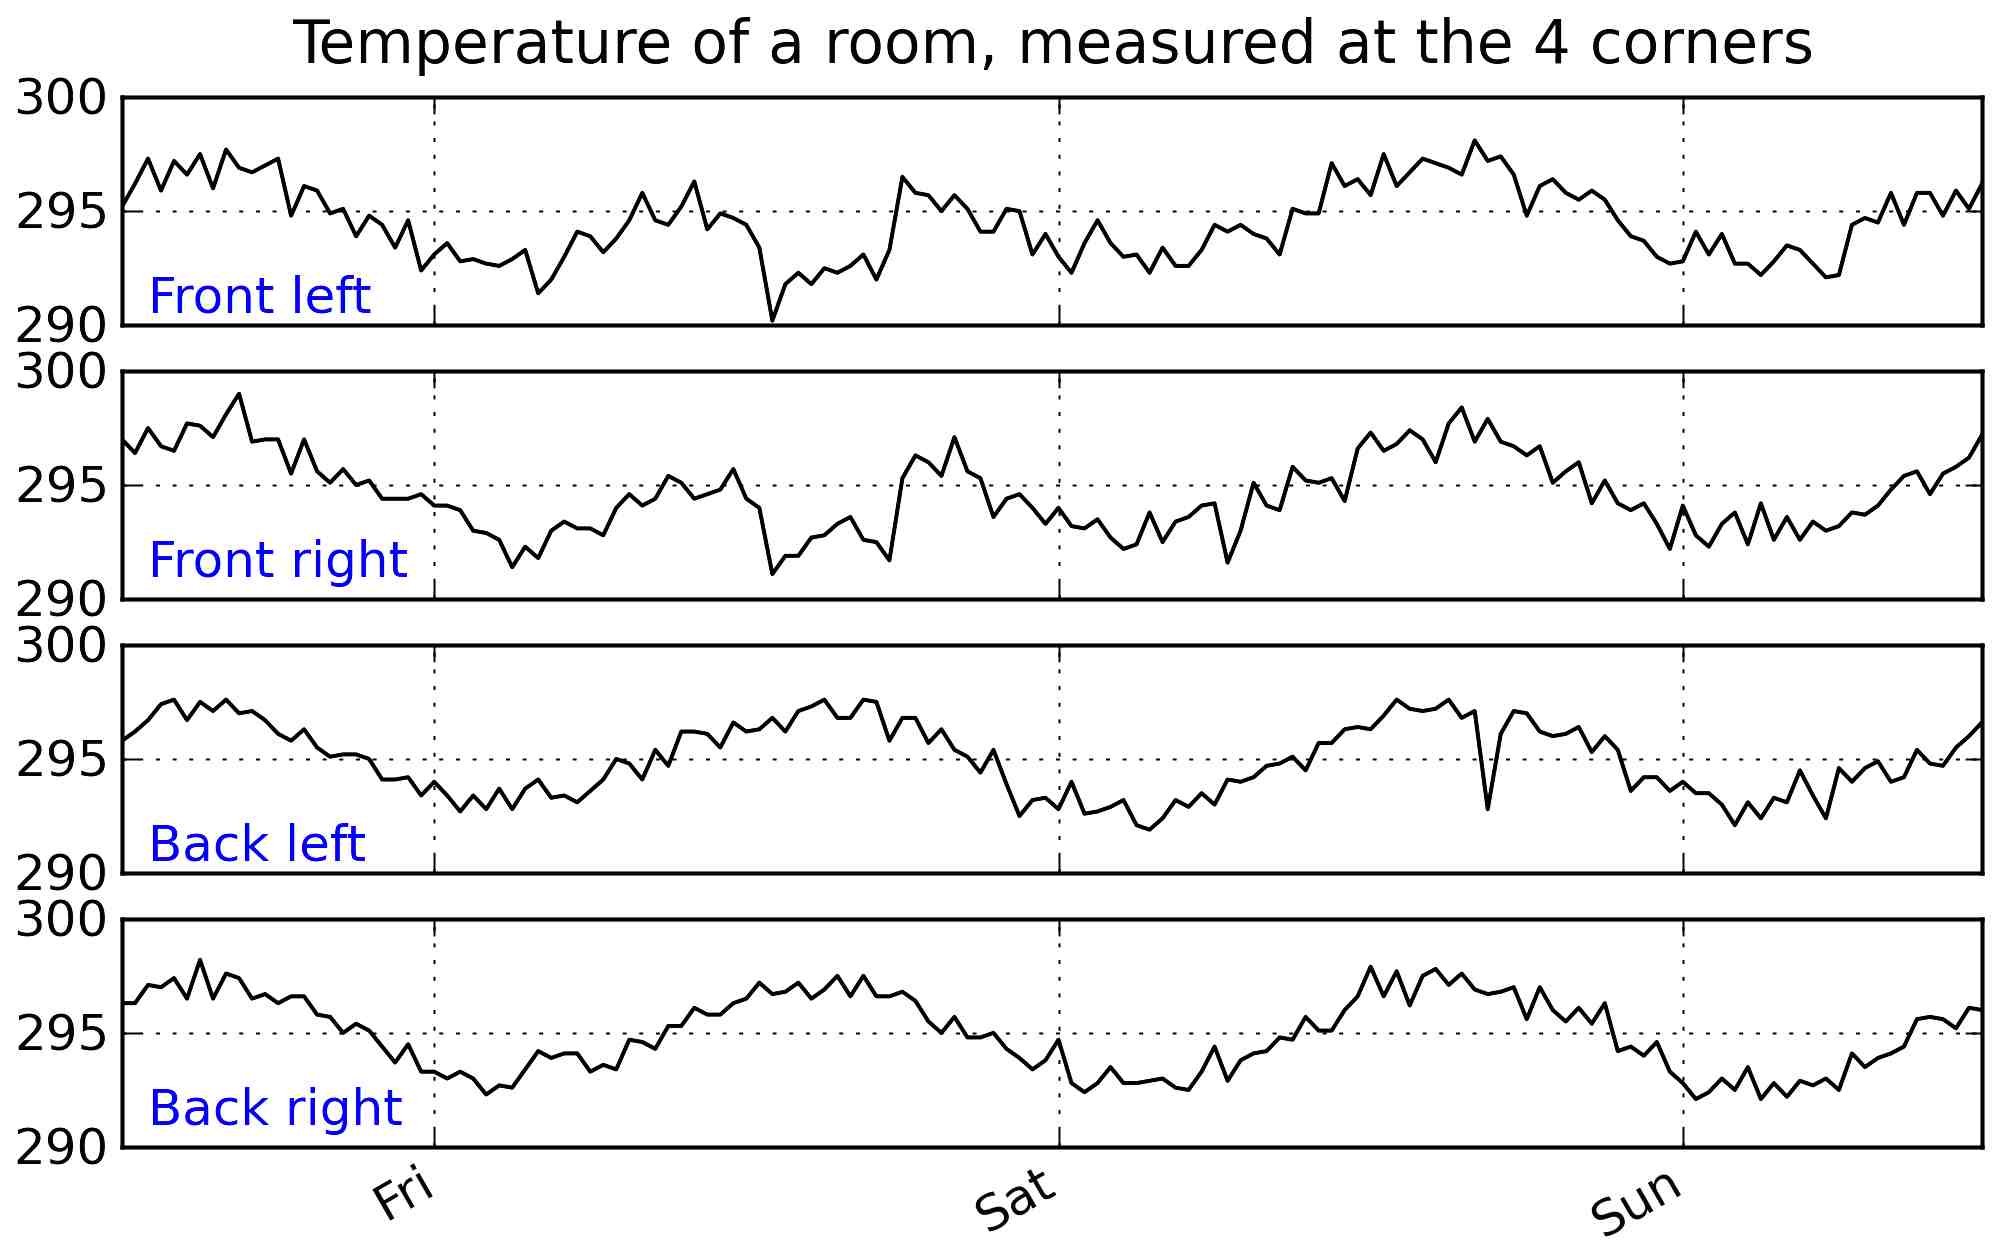
\includegraphics[width=6cm]{images/room-temperature-plots.jpg}
		% images/room-temperature-plots.py ---> PNG ---> cropped ---> saved as JPG
	\end{center}
	
	\begin{itemize}
		\item	a single phenomenon occurring, so \textbf{not 4 independent}  measurements
		
		\item	can be reduced down to 1 latent variable
		
				\begin{itemize}
					\item	just use the average
					
					\item	that's exactly what PCA does in this example
					
					\item	\( p_1 = [0.25,  0.25, 0.25, 0.25 ] \)
				\end{itemize}
		
	\end{itemize}
	
	
	% FUTURE: come back to pencil notes in Red McMaster Sketchbook binder and add the part that shows the weighted sum calculation for the scores

\end{frame}

\begin{frame}\frametitle{LV model outputs}

	\textbf{\emph{Example}}: room temperature measured at 4 points (contd)
	
	\begin{itemize}
		
		\item	How well did PCA do with 1 latent variable? Use \( R^2 \)
		
		\item	\vspace{6pt}\( R^2 = \frac{\displaystyle\text{Variability explained in}\,\, \hat{\mathbf{X}}}{\displaystyle \text{Variability started off with}} \) \vspace{6pt}
		
		\item	The part \emph{not explained}: called the error, \( \mathbf{E} \)
	\end{itemize}
	
	\begin{center}
		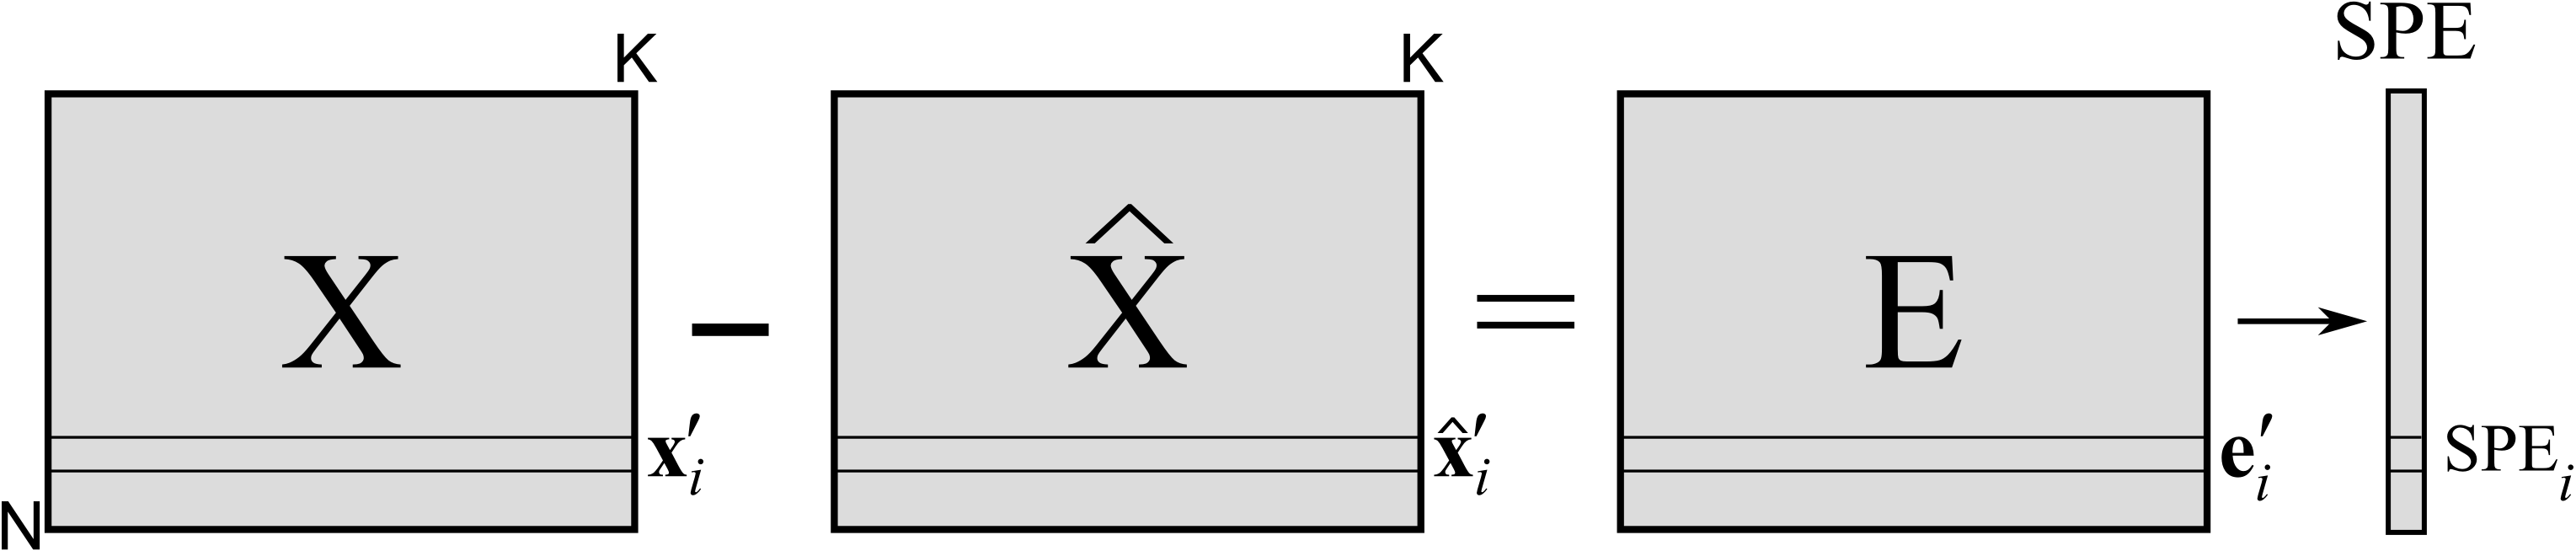
\includegraphics[width=\textwidth]{images/SPE-illustration.png}
	\end{center}

	\begin{itemize}
		\item	One SPE value per observation
	\end{itemize}
	
\end{frame}

\begin{frame}\frametitle{LV model outputs}

	\textbf{\emph{Example}}: room temperature measured at 4 points (contd)
	
	\begin{center}
		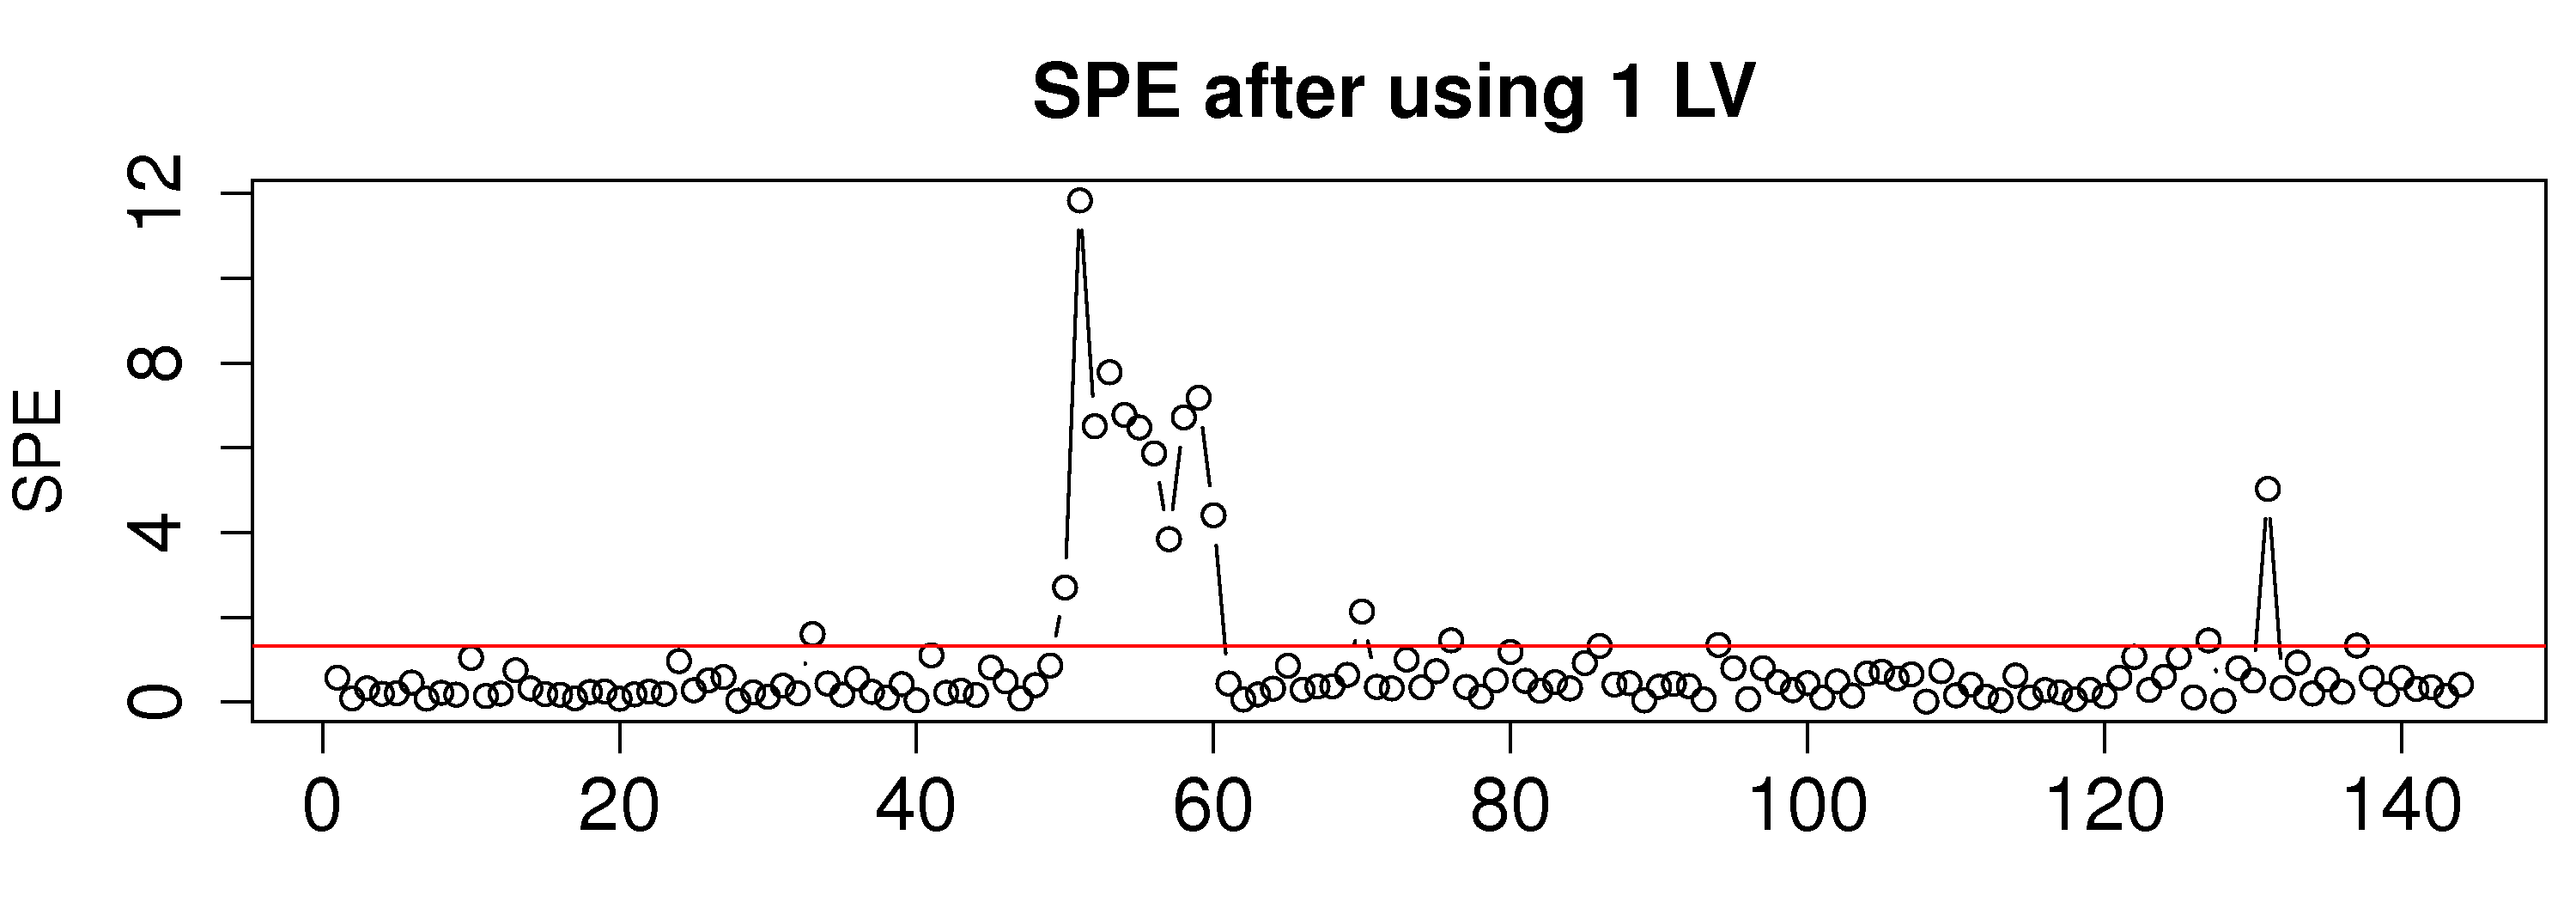
\includegraphics[width=\textwidth]{images/temperatures-SPE-after-one-PC.png}
		% From: /Users/kevindunn/ConnectMV/pid-book/latent-variable-modelling/images/temperature-data.R
	\end{center}

	Use SPE to:
	\begin{itemize}
		\item	verify whether there are unexplained features: add another component to capture
		
		\item	highlight outliers (unexplained, and unusual)
	\end{itemize}
	
\end{frame}

\begin{frame}\frametitle{LV model outputs}

	\textbf{\emph{Example}}: room temperature measured at 4 points (contd)
	
	\begin{center}
		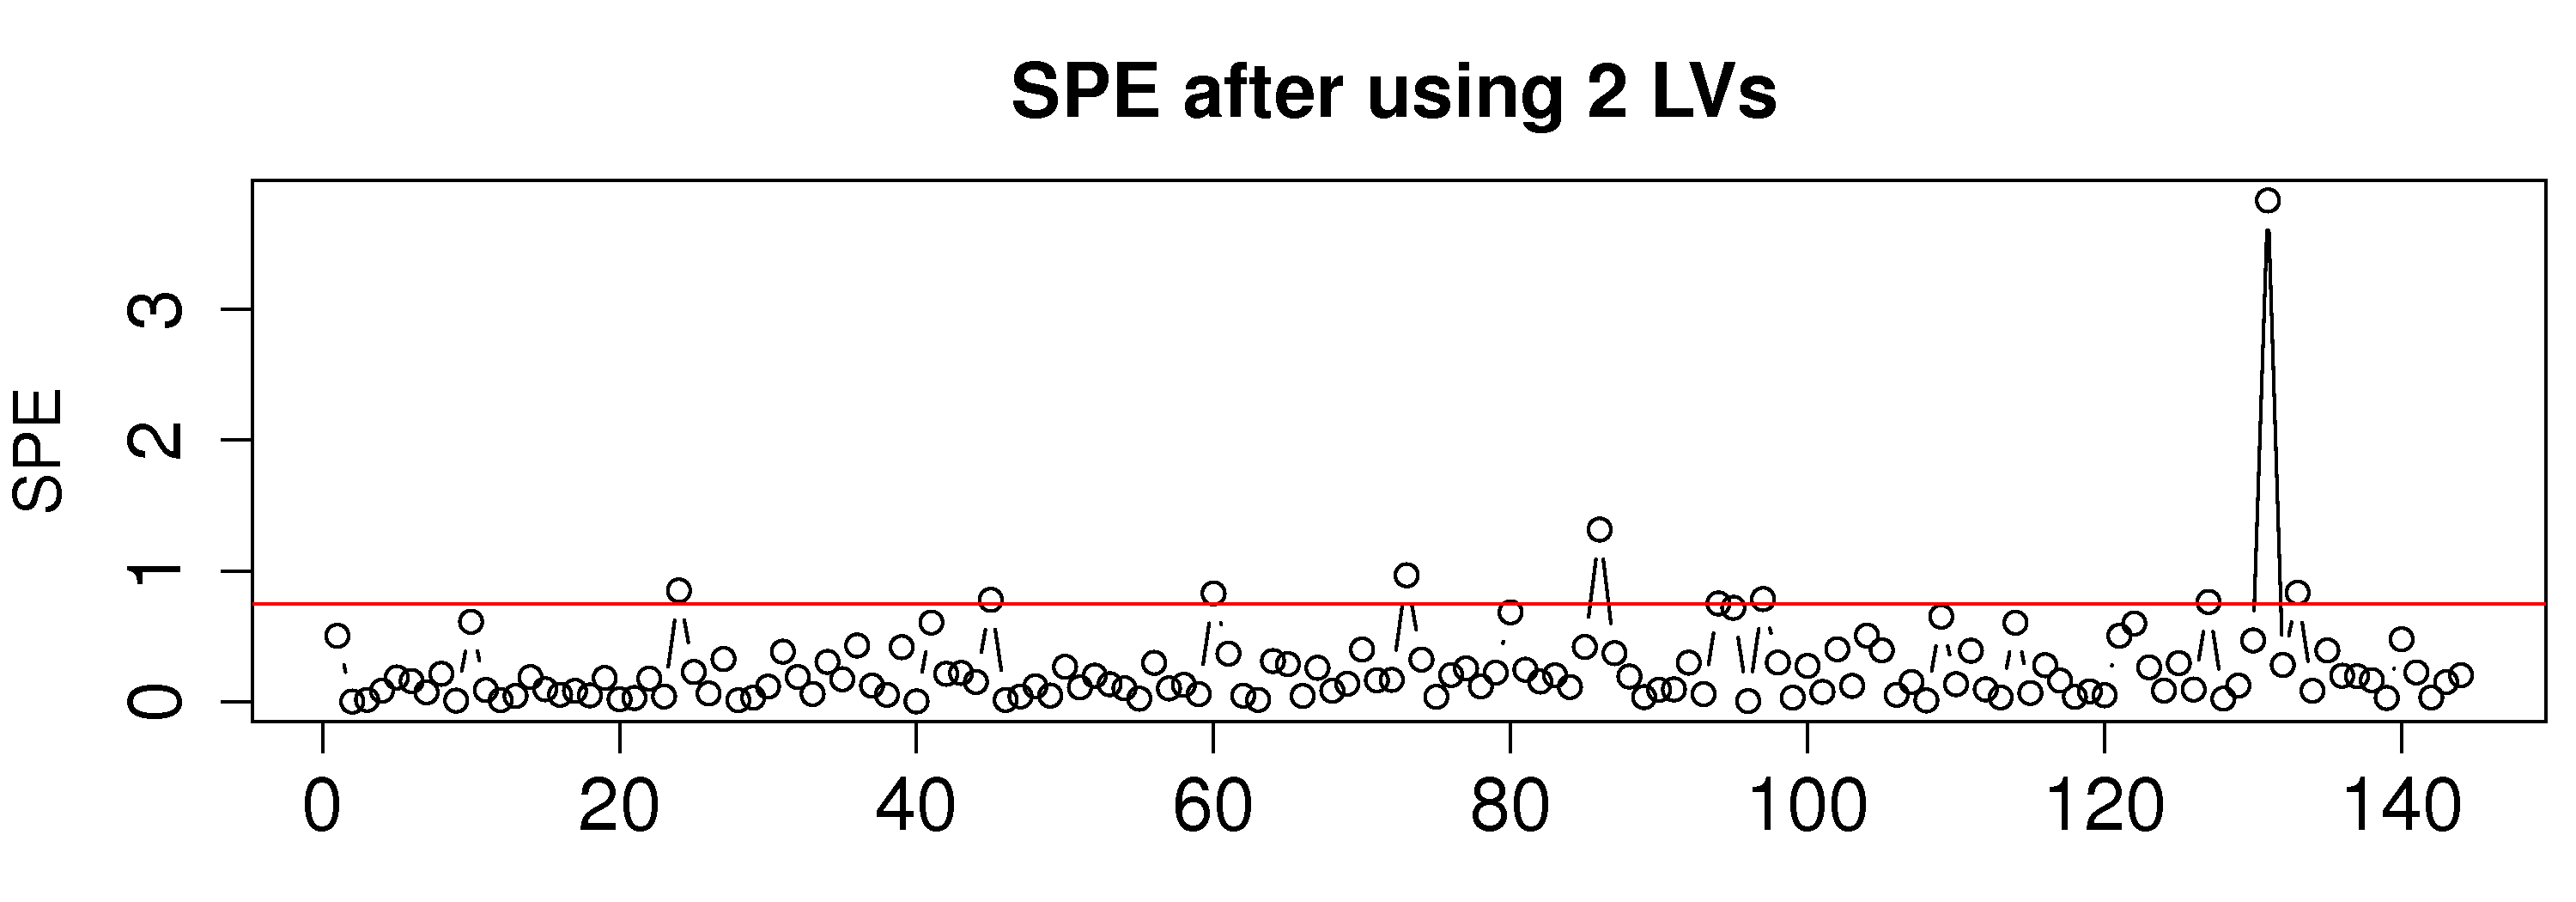
\includegraphics[width=\textwidth]{images/temperatures-SPE-after-two-LV.png}
		% From: /Users/kevindunn/ConnectMV/pid-book/latent-variable-modelling/images/temperature-data.R
	\end{center}

	\begin{itemize}
		\item	\( R^2_{a=1} = 76.6\% \)
		
		\item	\( R^2_{a=2} = 16.9\% \)
		
		\item	In general \( R^2_{a=1} > R^2_{a=2} > \ldots \)
	\end{itemize}
\end{frame}

\begin{frame}\frametitle{LV model outputs}

	\textbf{\emph{Example}}: room temperature measured at 4 points (contd)
	
	\begin{itemize}
		\item	An extra phenomenon in the data was modelled: can verify this with a \( t_2 \) plot
	\end{itemize}

	\begin{center}
		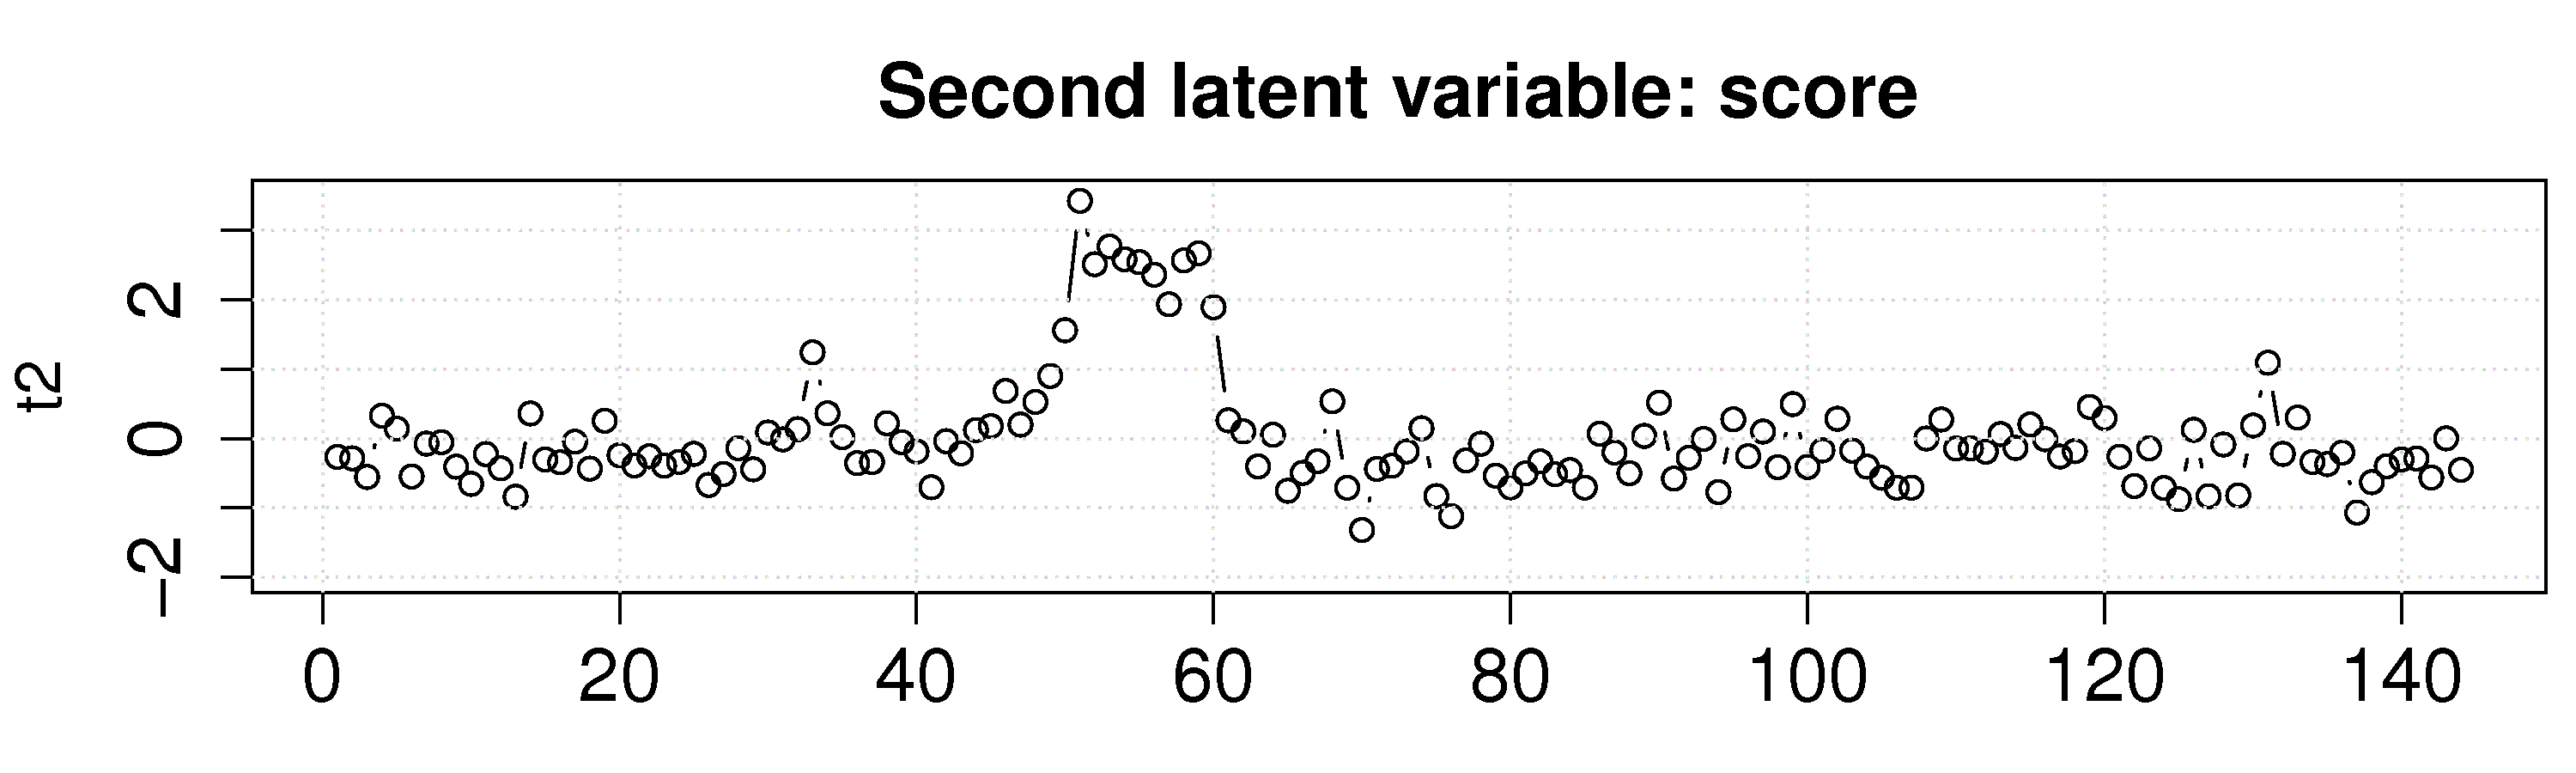
\includegraphics[width=\textwidth]{images/temperatures-LV-2-scores.png}
		% From: /Users/kevindunn/ConnectMV/pid-book/latent-variable-modelling/images/temperature-data.R
	\end{center}
\end{frame}

\begin{frame}\frametitle{Interpreting score plots: \(t_1, t_2, \ldots \)}

\begin{itemize}
	\item	Shown as scatter plot or time-series plot

	\item	Each point in plot is an observation

	\item	\(t_1\) explains more than \(t_2\); i.e. pay more attention to lower scores

		\begin{itemize}
			\item	observations that are similar appear close together in all scores
			\item	\emph{colour code} score plots by another variables: makes plot more informative
		\end{itemize}

\end{itemize}
\end{frame}

\begin{frame}\frametitle{Interpreting loading plots: \( p_1, p_2, \ldots \)}

\begin{itemize}
	
	\item	Shown as bar plots or scatter plots

	\item 	One point per variable (tag) in the model
	
			\begin{itemize}
				
				\item	Larger loadings more important than smaller loadings
				
			\end{itemize}

	\item 	Tags that behave similarly (move together) are close together 
	
\end{itemize}
\end{frame}

\begin{frame}\frametitle{Quick note on data preprocessing}

\begin{itemize}
	
	\item	Different units and scales coming together in one data set
	
	\item	Scaling: gives every variable fair representation in model
	
	\item	Centering: removes arbitrary offset (usually reduces model by 1 component)
	
\end{itemize}

\begin{center}
	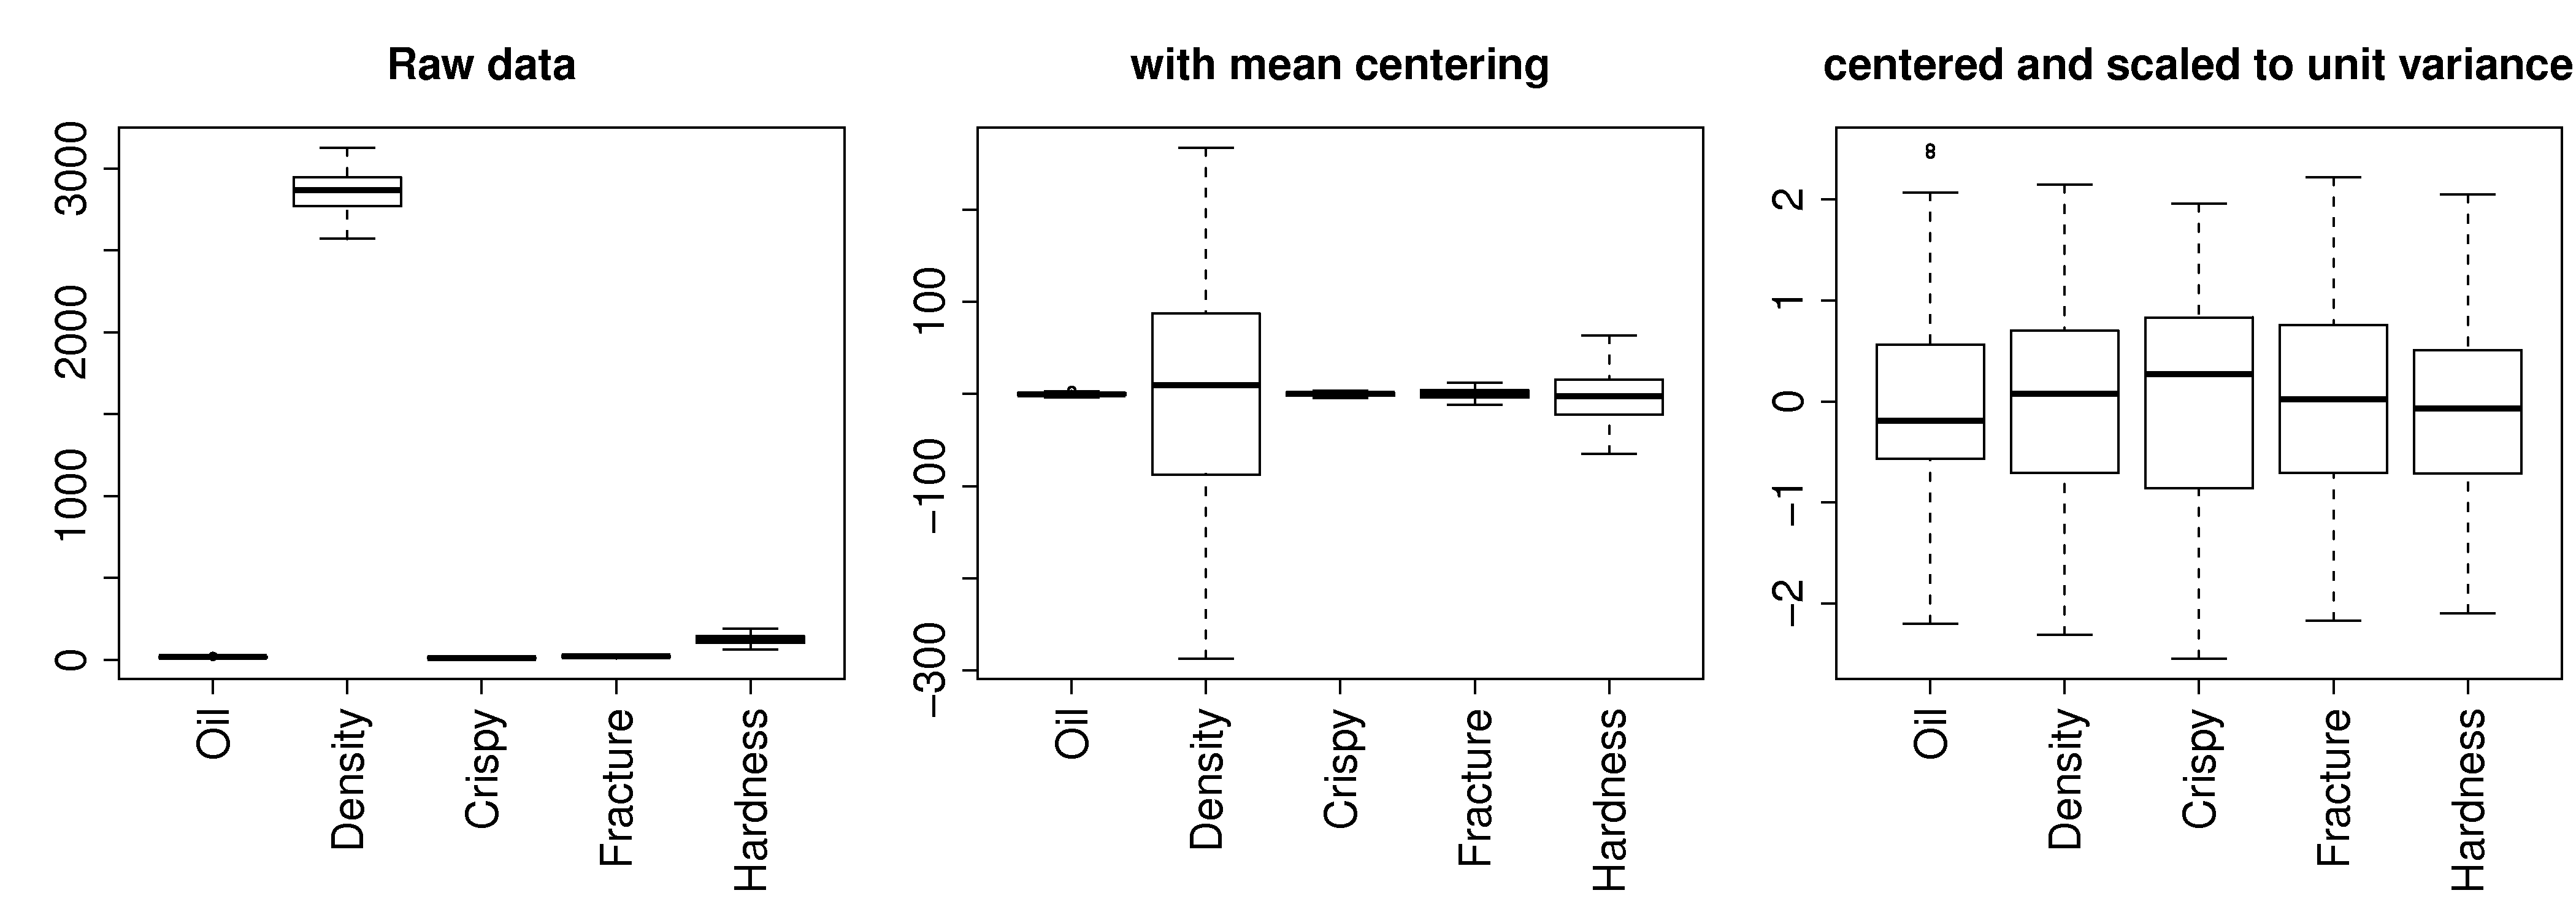
\includegraphics[width=\textwidth]{images/pca-on-food-texture-centering-and-scaling.png}
\end{center}
\end{frame}

